%-----------------------------------LICENSE------------------------------------%
%   This file is part of Mathematics-and-Physics.                              %
%                                                                              %
%   Mathematics-and-Physics is free software: you can redistribute it and/or   %
%   modify it it under the terms of the GNU General Public License as          %
%   published by the Free Software Foundation, either version 3 of the         %
%   License, or (at your option) any later version.                            %
%                                                                              %
%   Mathematics-and-Physics is distributed in the hope that it will be useful, %
%   but WITHOUT ANY WARRANTY; without even the implied warranty of             %
%   MERCHANTABILITY or FITNESS FOR A PARTICULAR PURPOSE.  See the              %
%   GNU General Public License for more details.                               %
%                                                                              %
%   You should have received a copy of the GNU General Public License along    %
%   with Mathematics-and-Physics.  If not, see <https://www.gnu.org/licenses/>.%
%------------------------------------------------------------------------------%

% Use the standalone class for displaying the tikz image on a small PDF.
\documentclass[crop, tikz]{standalone}

% Needed for mathbb.
\usepackage{amssymb}

% Import the tikz package to use for the drawing.
\usepackage{tikz}

% Load the arrows.meta library.
\usetikzlibrary{arrows.meta}

% Begin the document.
\begin{document}

    % Draw the figure.
    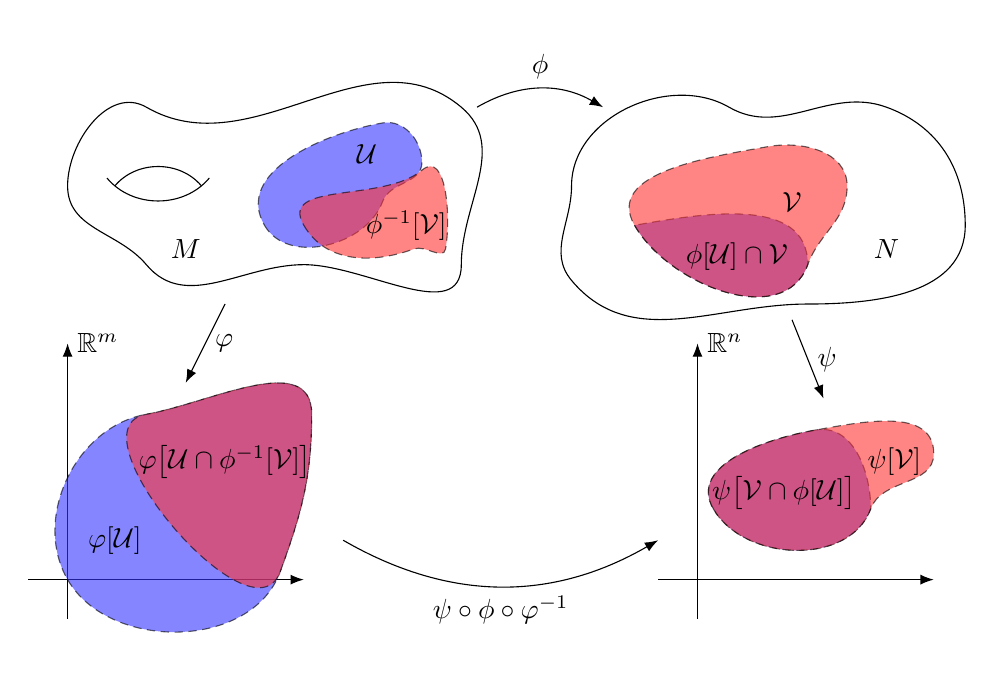
\begin{tikzpicture}[>=LaTeX]
        \draw (0.0, 0.0)    to[out=90,  in=150]  (1.0,  1.0)
                            to[out=-30, in=140]  (5.0,  1.0)
                            to[out=-40, in=90]   (5.0, -1.0)
                            to[out=-90, in=0]    (3.0, -1.0)
                            to[out=180, in=-50]  (1.0, -1.0)
                            to[out=130, in=-90]  cycle;

        \draw (0.5, 0.1) to[in=-130, out=-50] (1.8, 0.1);
        \draw (0.6, 0.0) to[in=130,  out=50]  (1.7, 0.0);

        \draw[fill=blue!80!white,opacity=0.6,densely dashed]
            (2.5, -0.5) to[out=-60,  in=-110] (4.0, -0.2)
                        to[out=70,   in=-90]  (4.5,  0.3)
                        to[out=90,   in=10]   (4.0,  0.8)
                        to[out=-170, in=120]  cycle;

        \draw[fill=red!80!white,opacity=0.6,densely dashed]
            (3.0, -0.5) to[out=-60,  in=-160] (4.4, -0.8)
                        to[out=20,   in=-100] (4.8, -0.8)
                        to[out=80,   in=40]   (4.5,  0.2)
                        to[out=-140, in=120]  cycle;

        \node at (3.8,  0.4) {$\mathcal{U}$};
        \node at (4.3, -0.5) {$\phi^{-1}[\mathcal{V}]$};
        \node at (1.5, -0.8) {$M$};

        \draw[->] (5.2, 1) to[out=30, in=150] node[above] {$\phi$} (6.8, 1);

        \begin{scope}[xshift=6.4cm]
            \draw (0.0, 0.0)    to[out=90,  in=150]  (2.0,  1.0)
                                to[out=-30, in=160]  (4.0,  1.0)
                                to[out=-20, in=90]   (5.0, -0.5)
                                to[out=-90, in=0]    (3.0, -1.5)
                                to[out=180, in=-50]  (0.0, -1.2)
                                to[out=130, in=-90]  cycle;

            \draw[fill=blue!80!white,opacity=0.6,densely dashed]
                (0.8, -0.5) to[out=-60,  in=-110] (3.0, -1.0)
                            to[out=90,   in=10]   cycle;

            \draw[fill=red!80!white,opacity=0.6,densely dashed]
                (0.8, -0.5) to[out=-60,  in=-110] (3.0, -1.0)
                            to[out=70,   in=-90]  (3.5,  0.0)
                            to[out=90,   in=10]   (2.5, 0.5)
                            to[out=-170, in=120]  cycle;

            \node at (4.0, -0.8) {$N$};
            \node at (2.8, -0.2) {$\mathcal{V}$};
            \node at (2.1, -0.9) {$\phi[\mathcal{U}]\cap\mathcal{V}$};
        \end{scope}

        \draw[->] (2.0, -1.5) to node[right] {$\varphi$} (1.5, -2.5);
        \begin{scope}[yshift=-5.0cm]
            \draw[->] (-0.5,  0.0) to (3.0, 0.0);
            \draw[->] ( 0.0, -0.5) to (0.0, 3.0) node[right] {$\mathbb{R}^{m}$};

            \draw[fill=blue!80!white,opacity=0.6,densely dashed]
                (0.0, 0.0) to[out=-60,  in=-110] (2.7, 0.1)
                           to[out=70,   in=-90]  (3.1, 2.1)
                           to[out=90,   in=10]   (1.0, 2.1)
                           to[out=-170, in=120]  cycle;

            \draw[fill=red!80!white,opacity=0.6,densely dashed]
                (2.7, 0.1) to[out=70,   in=-90]  (3.1, 2.1)
                           to[out=90,   in=10]   (1.0, 2.1)
                           to[out=-170, in=-110] cycle;

            \node at (0.6, 0.5) {$\varphi[\mathcal{U}]$};
            \node at (2.0, 1.5)
                {$\varphi\big[\mathcal{U}\cap\phi^{-1}[\mathcal{V}]\big]$};
        \end{scope}
        \draw[->] (9.2, -1.7) to node[right] {$\psi$} (9.6, -2.7);
        \begin{scope}[xshift=8.0cm,yshift=-5.0cm]
            \draw[->] (-0.5,  0.0) to (3.0, 0.0);
            \draw[->] ( 0.0, -0.5) to (0.0, 3.0) node[right] {$\mathbb{R}^{n}$};

            \draw[fill=blue!80!white,opacity=0.6,densely dashed]
                (1.5, 1.9) to[out=-170, in=120]  (0.2, 0.9)
                           to[out=-60,  in=-110] (2.2, 0.9)
                           to[out=90,   in=10]   cycle;

            \draw[fill=red!80!white,opacity=0.6,densely dashed]
                (0.2, 0.9) to[out=-60,  in=-110] (2.2, 0.9)
                           to[out=70,   in=-90]  (3.0, 1.6)
                           to[out=90,   in=10]   (1.5, 1.9)
                           to[out=-170, in=120]  cycle;

            \node at (2.5, 1.5) {$\psi[\mathcal{V}]$};
            \node at (1.1, 1.1) {$\psi\big[\mathcal{V}\cap\phi[\mathcal{U}]\big]$};
        \end{scope}
        \draw[->] (3.5, -4.5) to[out=-30, in=-150] node[below]
            {$\psi\circ\phi\circ\varphi^{-1}$} (7.5, -4.5);
    \end{tikzpicture}
\end{document}
